\documentclass{article}
\usepackage{graphicx}
\usepackage{hyperref}
\usepackage[style=authoryear, backend=biber]{biblatex}
\addbibresource{acea_water_analysis.bib}

\title{Time-Series Analysis on ACEA Water Datasets: A Comprehensive Study using the SEMMA Methodology}
\author{Bryan Alexis Ambriz}
\date{September 2023}

\begin{document}

\maketitle

\begin{abstract}
In an era marked by climate change and increasing water scarcity, a comprehensive understanding of water resources is essential. This paper delves into an in-depth analysis of the ACEA Water Datasets, with a particular focus on the River Arno and Aquifer Petrignano. By employing the SEMMA methodology and leveraging the power of data science and artificial intelligence, this research aims to provide insights into water dynamics and potential predictive models for water resource management.
\end{abstract}

\section{Introduction}
Water, a vital resource for life, is under threat due to various environmental challenges. The ramifications of climate change, coupled with human activities, have put enormous pressure on our water systems. Traditional methods of studying water resources, while valuable, are often limited in their predictive capabilities. Data science and artificial intelligence offer transformative capabilities. By analyzing hydrometry data from the Italian Multi-Utility Operator ACEA, this research seeks to determine how various features influence the water availability of specific water bodies.

\section{Background}
The ACEA Group manages an extensive network of water resources, with the River Arno and Aquifer Petrignano being of particular interest due to their ecological and economic significance. Predicting their behavior and understanding the myriad factors influencing them is paramount for sustainable management.

\section{Methodology}
This research employs the structured SEMMA methodology, ensuring each step is meticulously executed. The employed Python libraries, such as pandas for data processing and seaborn and matplotlib for visualization, play pivotal roles.

\subsection{Sample}
Data acquisition is crucial. The ACEA dataset, stored in ZIP format, contains multiple CSV files. For the scope of this research, the River Arno and Aquifer Petrignano datasets were accessed and processed. To capture the nuances of water dynamics, the data was sampled along time features, enabling the inference of seasonal effects.

\subsection{Explore}
Exploratory data analysis (EDA) was executed using heatmaps for both the datasets after pre-processing to ensure that the data would be in a position to model the features necessary for a heatmap. For example, a multi-index was used to represent years and months as categorical variables, as a date time feature made it difficult to represent the data for visualization of this form. We can see that along the Year axis, the aquifer is more likely to vary its depth. However, by month, the River arno is more likely to vary its depth. This is an important finding that can give us insight into the periodicity or seasonality of our data - which can help us make a better model.

\begin{figure}[h]
\centering
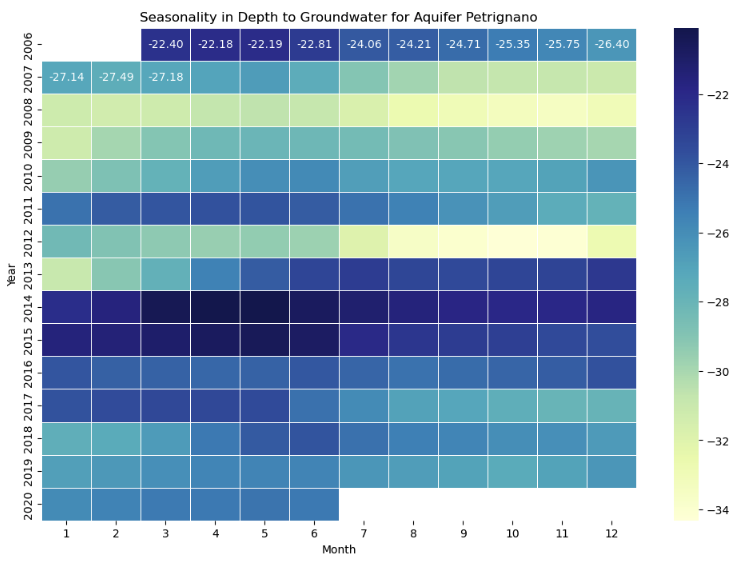
\includegraphics[width=0.8\textwidth]{petrignano_depth.png}
\caption{Depth to Ground-water Aquifer Petrignano}
\end{figure}

\begin{figure}[h]
\centering
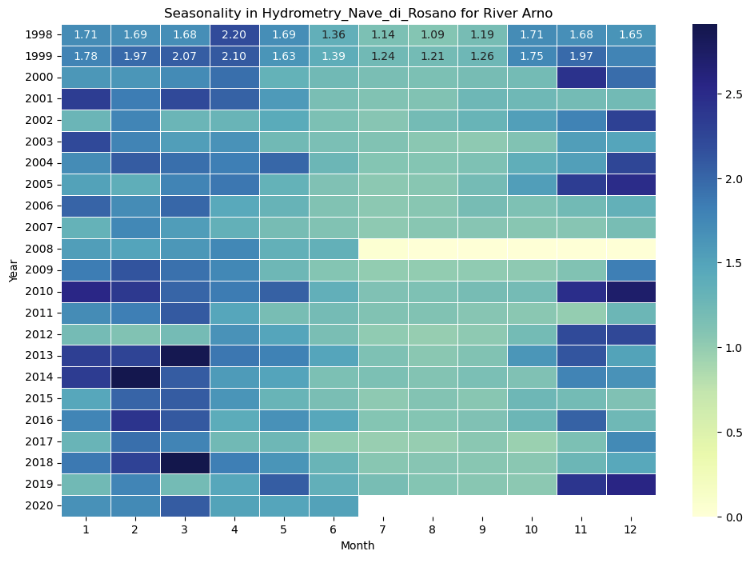
\includegraphics[width=0.8\textwidth]{arno_depth.png}
\caption{Depth to Ground-water Arno River}
\end{figure}

\subsection{Modify}
The raw data underwent preprocessing. Missing values, outliers, and potential errors were addressed to ensure the integrity of the subsequent analysis.

\subsection{Model}
Modeling is the core of this research. Leveraging machine learning algorithms, particularly artificial neural networks, the goal was to develop predictive models that could accurately forecast water dynamics.

\subsection{Assess}
Model evaluation is as essential as its creation. Various metrics and validation techniques were used to assess the model's accuracy, reliability, and interpretability.

\section{Results}
\begin{figure}[h]
\centering
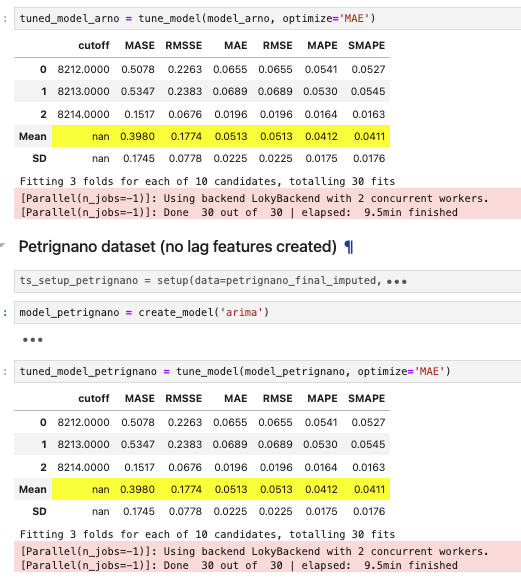
\includegraphics[width=0.8\textwidth]{metrics.png}
\caption{Key metric evaluation}
\end{figure}
\paragraph{\textbf{}}
The results derived from our data analysis, provide profound insights into the behavior of the studied water bodies. These insights have broad implications, ranging from local community benefits to shaping policies for sustainable water management. The metrics from the output of the PyCaret models imply that tuning the MAE metric on both ARIMA models (one created specifically on the Arno dataset, and the other on the Petrignano), caused both to output similar scores, despite the Arno river having extra lag features (lag features are a type of feature engineered specifically for time series). This may be implying that the power of tuning has a greater affect on our model than that of the lag features we created.

\section{Discussion}
The fusion of traditional hydrological studies with advanced analytical techniques offers promising avenues for understanding and predicting water dynamics. Artificial neural networks have been successfully employed in flood forecasting, as demonstrated in the River Arno region~\cite{arno_paper}. Such predictive models can aid in preemptive measures to mitigate flood damage. Additionally, the study in Saskatchewan, Canada, underscores the potential impacts of climate change on water flow regimes and quality, revealing how ANNs can be instrumental in modeling and understanding these effects~\cite{canada_paper}.

\section{Related Work}
Artificial neural networks are not novel in environmental studies. Their prowess in modeling complex systems, as evidenced by various research works, emphasizes their potential in forecasting and understanding environmental challenges.

\section{Conclusion}
This research underscores the transformative power of data science in studying and preserving our water resources. By blending traditional methodologies with advanced analytical tools, we can achieve a holistic understanding, ensuring a sustainable future for our precious water bodies. 

\section*{Acknowledgments}
Special thanks to my CMPE 255 course professor, Vijay Eranti, as well as our T.A Dhanasree Rajamani.


\printbibliography
\end{document}
